% Provenance (never printed): see sources/outline_sources.md (Year 1: rigid plates on a
% sphere, Euler poles and angular velocities; relative velocities; triple junctions;
% finite rotations; the magnetic-anomaly timescale; satellite geodesy). Curves and maps
% from figdata/bachelor-1/euler_velocities.py, south_atlantic_fit.py and gpts_stripes.py;
% exercise and problem values in the Book 3 scratch calculator calc/ch12.py.
\chapter{حركيّة الصفائح على الكرة}\label{ch:b1:plate-kinematics}

منذ أكثر من ربع قرن تسجّل محطتان لتحديد المواقع بالأقمار الصناعية موقعهما كل يوم: إحداهما في ريكيافيك، غرب أيسلندا، والأخرى قرب ستافانغر على الساحل الغربي للنرويج. والخط المستقيم بينهما، الذي يبلغ طوله \qty{1546}{km}، يزداد بمقدار \qty{17.5}{mm} كل سنة، أي نحو سنتيمترين. ولا شيء على الأرض يُظهر ذلك، ومع ذلك يسجّل قاع المحيط الأطلسي الشمالي بين المحطتين الاتساع نفسه على مدى ملايين السنين: فالحمم التي تثور عند الحيد الأطلسي الأوسط تأخذ اتجاه المجال المغناطيسي للأرض وهي تبرد، والمجال انعكس مرارًا، فيحمل قاع المحيط سجلًا مخطّطًا لنموّه. يحوّل هذا الفصل صفائح سنوات الدراسة إلى أغطية صلبة على كرة، ويصف حركاتها بهندسة الدورانات، ويبيّن كيف يقيس السجل الجيولوجي والأقمار الصناعية الحركات نفسها.
% ledger: ngl:reyk, ngl:stas (chord lengthening computed in calc/ch12.py)

\begin{recall}
على الكرة، \omterm{def:b1:spherical-astronomy:spherical-triangle}{الدائرة العظمى} هي تقاطع الكرة مع مستوٍ يمرّ بمركزها، \omterm{def:b1:spherical-astronomy:spherical-triangle}{والدائرة الصغرى} تقاطعها مع أي مستوٍ آخر؛ ومبرهنة جيب التمام تعطي المسافة الزاوية بين نقطتين من عرضيهما وطوليهما، ويُعدّ \omterm{def:b1:spherical-astronomy:horizontal}{السمت} لاتجاه ما من الشمال نحو الشرق (\cref{ch:b1:spherical-astronomy}). والجسم الصلب الذي يدور حول محور ثابت له سرعة زاوية (الفيزياء). ويتجزّأ \omterm{def:b1:layered-earth:lithosphere}{الغلاف الصخري} إلى صفائح تتحرّك بعضها بالنسبة إلى بعض بسرعات بضعة سنتيمترات في السنة، ويحمل قاع المحيط خطوطًا مغناطيسية تسجّل انعكاسات المجال المغناطيسي للأرض (الكتاب 2، الصف 11).
\end{recall}

\section{صفائح صلبة على كرة}

تمتد صفيحة على جزء كبير من الكرة: فالصفيحة الأوراسية تمتد من وسط الأطلسي إلى شرق سيبيريا. ولا يمكن وصف حركتها بسرعة، كما تُوصف حركة السيارة، بل يجب وصفها بدوران.

\begin{definition}[الصفيحة الصلبة]\label{def:b1:plate-kinematics:rigid-plate}
\emph{الصفيحة الصلبة}\index{الصفيحة الصلبة} هي منطقة من \omterm{def:b1:layered-earth:lithosphere}{الغلاف الصخري} لا يتشوّه داخلها تشوّهًا قابلًا للقياس: فالمسافة بين أي نقطتين منها تبقى ثابتة. وتُمتص الحركة النسبية لصفيحتين على حدّهما المشترك، وهو منطقة ضيقة من الصدوع والزلازل والبراكين.
\end{definition}

لا توجد صفيحة صلبة تمامًا: فالحدود مناطق عرضها عشرات إلى مئات الكيلومترات، والأجزاء الداخلية تتشوّه ببطء. والفرضية أن هذه الانحرافات صغيرة قياسًا إلى الحركات النسبية؛ ويُختبر ذلك باتساق كل نتيجة في هذا الفصل.

تتحرّك \omterm{def:b1:plate-kinematics:rigid-plate}{الصفيحة الصلبة} على سطح كرة دون أن تتغيّر المسافة بين أي نقطتين منها، ومركز الأرض لا يتحرّك. ويوصف هذا الانتقال بمصفوفة $3\times3$ هي $R$ تحفظ الأطوال، وهي مصفوفة \emph{متعامدة} ($R^{\mathsf T}R = I$)، وتحفظ اتجاه الفضاء، فيكون $\det R = 1$: تنتقل نقطة متجهها الموضعي $\vec r$ إلى $R\vec r$.

\begin{theorem}[مبرهنة دوران أويلر]\label{thm:b1:plate-kinematics:euler}
كل إزاحة \omterm{def:b1:plate-kinematics:rigid-plate}{لالصفيحة الصلبة} على الكرة هي دوران حول محور يمرّ بمركز الأرض: يوجد متجهة وحدة $\vec n$ بحيث $R\vec n = \vec n$، وتدور الصفيحة حول $\vec n$ بزاوية ما.
\end{theorem}

\begin{proof}
نُثبت أن $1$ قيمة ذاتية للمصفوفة $R$، أي $\det(R - I) = 0$. ولما كان $R R^{\mathsf T} = I$ فإن $R - I = R(I - R^{\mathsf T})$، ومنه
\[
  \det(R - I) = \det R\,\det\bigl((I - R)^{\mathsf T}\bigr) = \det(I - R),
\]
باستعمال $\det R = 1$، وكون المصفوفة ومنقولتها لهما المحدِّد نفسه. وبالنسبة إلى مصفوفة $3\times3$ يكون
$\det(I - R) = (-1)^3\det(R - I) = -\det(R - I)$. إذن $\det(R - I) =
-\det(R - I)$، وهذا يساوي صفرًا. فتوجد إذن متجهة وحدة $\vec n$ بحيث $R\vec n = \vec n$: فالنقطتان اللتان يلتقي عندهما الخط المار بالمركز في اتجاه $\vec n$ مع السطح لا تتحركان. وفي المستوي العمودي على $\vec n$ تحفظ $R$ الأطوال والاتجاه، فتديره بزاوية ما، فتدير الكرة كلها حول $\vec n$.
\end{proof}

خلال فترة زمنية قصيرة بما يكفي لئلا تتغيّر الحركة، يسير الدوران بمعدّل ثابت، وتكون الحركة النسبية لصفيحة بالنسبة إلى أخرى سرعةً زاويةً حول محور ثابت.

\begin{definition}[قطب أويلر؛ متجهة أويلر]\label{def:b1:plate-kinematics:euler-pole}
حركة الصفيحة B بالنسبة إلى الصفيحة A دوران حول محور يمرّ بمركز الأرض. و\emph{قطب أويلر}\index{قطب أويلر} للزوج هو النقطة التي يلتقي عندها هذا المحور بالسطح، مختارةً بحيث يكون الدوران عكس عقارب الساعة منظورًا من فوقها؛ والنقطة المقابلة هي القطب المضادّ. و\emph{متجهة أويلر}\index{متجهة أويلر} $\vec\omega_{BA}$ هي السرعة الزاوية للصفيحة B بالنسبة إلى A: تتجه من مركز الأرض نحو قطب أويلر، وطولها $\omega$ هو معدّل الدوران.
\end{definition}

تُعطى \omterm{def:b1:plate-kinematics:euler-pole}{متجهة أويلر} بعرض قطبها الجغرافي وطوله ومعدّل دورانها، ويُعبَّر عن المعدّل عادةً بالدرجات في المليون سنة. وحركة الصفيحة الأوراسية بالنسبة إلى الصفيحة الأمريكية الشمالية، متوسطةً على آخر \qty{3.16}{Myr} من 453 معدّل انتشار قيس على الحيود بينهما، لها قطب عند \ang{61.8}~ش، و\ang{139.6}~ق، في شرق سيبيريا، ومعدّل \qty{0.210}{\degree\per\Myr}. وبالراديان في السنة،
\[
  \omega = \frac{0.210\times\pi/180}{\num{e6}} = \qty{3.665e-9}{rad.yr^{-1}},
\]
أي دورة كاملة في \qty{1714}{\Myr}.
% ledger: morvel:eu-na, morvel:summary

\section{السرع النسبية}

\begin{theorem}[السرعة على صفيحة دوّارة]\label{thm:b1:plate-kinematics:velocity}
إذا دارت الصفيحة B بالنسبة إلى الصفيحة A \omterm{def:b1:plate-kinematics:euler-pole}{بمتجهة أويلر} $\vec\omega$، فإن نقطة من B متجهها الموضعي $\vec r$ (من مركز الأرض) تتحرّك بالنسبة إلى A بالسرعة
\[
  \vec v = \vec\omega\times\vec r .
\]
\end{theorem}

\begin{proof}
ليكن $\Delta$ الزاوية بين $\vec\omega$ و$\vec r$. وعند دوران B تصف النقطة دائرة حول المحور، نصف قطرها $R\sin\Delta$، حيث $R$ نصف قطر الأرض؛ وبالمعدّل الزاوي $\omega$ تكون سرعتها $\omega R\sin\Delta$. وسرعتها مماسّة لتلك الدائرة، فهي عمودية على المحور وعلى نصف القطر $\vec r$ معًا، وبما أن الدوران عكس عقارب الساعة حول $\vec\omega$، فإن اتجاهها هو اتجاه $\vec\omega\times\vec r$. وللمتجهة $\vec\omega\times\vec r$ هذا الاتجاه والمعنى بالضبط، وطولها $\omega R\sin\Delta$.
\end{proof}

والزاوية $\Delta$ هي المسافة الزاوية بين \omterm{def:b1:plate-kinematics:euler-pole}{قطب أويلر} والنقطة، وتعطيها مبرهنة جيب التمام من العرض والطول.

\begin{proposition}[السرعة النسبية واتجاه الحركة]\label{prop:b1:plate-kinematics:speed}
ليكن \omterm{def:b1:plate-kinematics:euler-pole}{قطب أويلر} عند \omterm{def:b1:spherical-astronomy:geographic}{العرض الجغرافي} $\varphi_p$ والطول $\lambda_p$، والنقطة عند $\varphi$ و$\lambda$. عندئذٍ
\begin{enumerate}
  \item المسافة الزاوية $\Delta$ من القطب إلى النقطة تحقّق $\cos\Delta = \sin\varphi_p\sin\varphi + \cos\varphi_p\cos\varphi
        \cos(\lambda - \lambda_p)$؛
  \item السرعة النسبية هي $v = \omega R\sin\Delta$: معدومة عند القطب، وأكبر ما تكون، أي $\omega R$، على \omterm{def:b1:spherical-astronomy:spherical-triangle}{الدائرة العظمى} التي تبعد عنه \ang{90}؛
  \item اتجاه الحركة عمودي على \omterm{def:b1:spherical-astronomy:spherical-triangle}{الدائرة العظمى} التي تصل النقطة بالقطب: وسمتها هو \omterm{def:b1:spherical-astronomy:horizontal}{سمت القطب} كما يُرى من النقطة، زائدًا \ang{90}.
\end{enumerate}
\end{proposition}

\begin{proof}
(1) هي مبرهنة جيب التمام في \omterm{def:b1:spherical-astronomy:spherical-triangle}{المثلث الكروي} الذي تكوّنه القطب الشمالي الجغرافي \omterm{def:b1:plate-kinematics:euler-pole}{وقطب أويلر} والنقطة، وضلعاه من القطب الشمالي هما $\ang{90} - \varphi_p$ و$\ang{90} - \varphi$، والزاوية بينهما $\lambda - \lambda_p$. و(2) تنتج من المبرهنة. و(3) السرعة عمودية على $\vec\omega$ وعلى $\vec r$، فهي عمودية على المستوي الذي يحويهما، أي مستوي \omterm{def:b1:spherical-astronomy:spherical-triangle}{الدائرة العظمى} المارة بالنقطة والقطب. وفي المستوي الأفقي عند النقطة تكون إذن عمودية على اتجاه القطب؛ ولأن الدوران عكس عقارب الساعة منظورًا من فوق القطب، فإن النقطة تتحرك إلى يمين الاتجاه الذي تراه فيه القطب، وهذا يضيف \ang{90} إلى \omterm{def:b1:spherical-astronomy:horizontal}{السمت}.
\end{proof}

\begin{omfigure}
\begin{tikzpicture}[x=2.5cm, y=2.5cm, font=\scriptsize, >=Stealth]
% orthographic view from 20 deg above the "Euler equator": a point at polar angle D,
% longitude p about the pole projects to X = sin D sin p, Y = cos D cos 20 - sin D cos p sin 20;
% it is visible when cos p >= -cot D tan 20 (limits computed by hand: 129.08, 102.13, 90, 77.87)
\fill[omSea!12] (0,0) circle (1);
\draw[thick] (0,0) circle (1);
\foreach \D/\m in {30/129.08, 60/102.13, 90/90, 120/77.87} {
  \draw[blue!45!black, domain=-\m:\m, samples=60, variable=\p]
    plot ({sin(\D)*sin(\p)}, {cos(\D)*cos(20) - sin(\D)*cos(\p)*sin(20)});
  \draw[blue!45!black, densely dashed, domain=\m:360-\m, samples=60, variable=\p]
    plot ({sin(\D)*sin(\p)}, {cos(\D)*cos(20) - sin(\D)*cos(\p)*sin(20)});
}
\draw[densely dashed] (0,0) -- (0,0.9397);
\draw[->, very thick] (0,0.9397) -- (0,1.38) node[above] {$\vec\omega$};
\fill (0,0.9397) circle (0.9pt) node[anchor=south west] {قطب أويلر};
\fill (0,0) circle (0.7pt);
% velocity arrows at longitude -35 deg about the pole, length 0.5 sin D
\draw[->, very thick, red!75!black] (-0.287,0.6737) -- ++(0.243,-0.058);
\draw[->, very thick, red!75!black] (-0.497,0.2272) -- ++(0.421,-0.101);
\draw[->, very thick, red!75!black] (-0.574,-0.2802) -- ++(0.487,-0.117);
\draw[->, very thick, red!75!black] (-0.497,-0.7124) -- ++(0.421,-0.101);
\draw[->] (0,0) -- (-0.497,0.2272) node[pos=0.55, below] {$\vec r$};
\draw (0,0.22) arc[start angle=90, end angle=155.4, radius=0.22];
\node at (-0.11,0.33) {$\Delta$};
\node[anchor=west] at (0.62,0.81) {$\Delta = \ang{30}$};
\node[anchor=west] at (0.88,0.47) {$\Delta = \ang{60}$};
\node[anchor=west] at (1.02,0.0) {$\Delta = \ang{90}$};
\node[anchor=west] at (0.88,-0.47) {$\Delta = \ang{120}$};
\end{tikzpicture}

\par\smallskip{\small صفيحة تدور حول \omterm{def:b1:plate-kinematics:euler-pole}{قطب أويلر}، منظورةً من نقطة قليلًا فوق الدائرة التي تبعد \ang{90} عن القطب. تتحرّك كل نقطة على \omterm{def:b1:spherical-astronomy:spherical-triangle}{الدائرة الصغرى} حول القطب (الأجزاء المخفية متقطّعة)؛ وسرعتها، التي تبيّنها الأسهم الحمراء، هي $\omega R\sin\Delta$، حيث $\Delta$ بعدها الزاوي عن القطب: معدومة عند القطب، وأكبر ما تكون على بعد \ang{90}.}
\label{fig:b1:plate-kinematics:euler-pole}
\end{omfigure}

لذلك تتغيّر سرعة الحركة النسبية على طول حدّ الصفيحة حتى لو كانت الصفيحتان صلبتين تمامًا، ويدور اتجاه الحركة معها. ونتيجتان تشكّلان كل خريطة لحدود الصفائح.

\begin{proposition}[الصدوع التحويلية تتبع الدوائر الصغرى]\label{prop:b1:plate-kinematics:transforms}
الصدع التحويلي، الذي تنزلق عنده صفيحتان بجوار بعضهما دون أن تتباعدا أو تتقاربا، يقع على \omterm{def:b1:spherical-astronomy:spherical-triangle}{الدائرة الصغرى} حول \omterm{def:b1:plate-kinematics:euler-pole}{قطب أويلر} للصفيحتين. ويكون اتجاه الانتشار عند حيد، واتجاه التقارب عند منطقة الاندساس، على الدوائر الصغرى كذلك.
\end{proposition}

\begin{proof}
عند صدع تحويلي تكون السرعة النسبية موازية للصدع في كل نقطة. والسرعة النسبية مماسّة في كل مكان للدوائر الصغرى حول القطب (\cref{thm:b1:plate-kinematics:velocity})؛ ومنحنٍ يماسّ عند كل نقطة منه \omterm{def:b1:spherical-astronomy:spherical-triangle}{الدائرة الصغرى} المارة بتلك النقطة هو إحدى هذه الدوائر. أما الجزء الثاني فهو الجزء الثالث من \cref{prop:b1:plate-kinematics:speed}.
\end{proof}

يتألّف حيد الأطلسي الأوسط بين أوراسيا وأمريكا الشمالية من درج من قطع حيدية تزيحها صدوع تحويلية؛ وتتّجه الصدوع التحويلية قرب الأسمات التي تتنبأ بها \omterm{def:b1:plate-kinematics:euler-pole}{متجهة أويلر}، وتُعدّ اتجاهاتها أحد المعطيات المستعملة لتحديد القطب. ويزداد معدّل الانتشار على طول الحدّ نفسه مع المسافة الزاوية من القطب: \qtyrange{11}{12}{mm.yr^{-1}} على حيد غاكيل في المحيط المتجمد الشمالي، قرب القطب، و\qty{23}{mm.yr^{-1}} شمال جزر الأزور مباشرةً، على بعد \ang{78} منه. ويقارن الشكل أدناه المعدّلات التي تتنبأ بها \omterm{def:b1:plate-kinematics:euler-pole}{متجهة أويلر} على امتداد الحدّ كله مع معدّلات نموذج صفائح مستقل.
% ledger: morvel:eu-na

\begin{method}[السرعة عند نقطة]\label{met:b1:plate-kinematics:velocity}
\begin{enumerate}
  \item حوّل معدّل \omterm{def:b1:plate-kinematics:euler-pole}{متجهة أويلر} إلى راديانات في السنة، واحسب $\omega R$ بوحدة \unit{mm.yr^{-1}} مع $R = \qty{6371}{km}$.
  \item احسب المسافة الزاوية $\Delta$ من القطب إلى النقطة بمبرهنة جيب التمام؛ والسرعة هي $\omega R\sin\Delta$.
  \item احسب \omterm{def:b1:spherical-astronomy:horizontal}{سمت القطب} كما يُرى من النقطة، $\beta$، مع
        $\tan\beta = \sin(\lambda_p - \lambda)\cos\varphi_p /
        \bigl(\cos\varphi\sin\varphi_p - \sin\varphi\cos\varphi_p
        \cos(\lambda_p - \lambda)\bigr)$، مع ربع البسط والمقام؛ والحركة نحو $\beta + \ang{90}$.
  \item تحقّق من الاتجاه: فالحركة هي حركة الصفيحة الثانية بالنسبة إلى الأولى. وتبادل الصفيحتين يعكسها.
\end{enumerate}
\end{method}

\begin{example}[أوراسيا تبتعد عن أمريكا الشمالية في أيسلندا]\label{ex:b1:plate-kinematics:iceland}
خذ منتصف أيسلندا عند \ang{64.5}~ش و\ang{18}~غ، \omterm{def:b1:plate-kinematics:euler-pole}{ومتجهة أويلر} لأوراسيا بالنسبة إلى أمريكا الشمالية المذكورة أعلاه. عندئذٍ $\omega R =
\num{3.665e-9}\times\qty{6.371e9}{mm} = \qty{23.35}{mm.yr^{-1}}$، و
\[
  \cos\Delta = \sin\ang{61.8}\sin\ang{64.5}
  + \cos\ang{61.8}\cos\ang{64.5}\cos(\ang{-18} - \ang{139.6}) = 0.60736,
\]
فيكون $\Delta = \ang{52.60}$ و$v = 23.35\sin\ang{52.60} = \qty{18.55}{mm.yr^{-1}}$.
يُرى القطب \omterm{def:b1:spherical-astronomy:horizontal}{بالسمت} $\beta = \ang{13.1}$، أي قليلًا شرق الشمال، فوق المحيط المتجمد الشمالي؛ وتتحرّك أوراسيا نحو $\ang{103.1}$، أي نحو الشرق الجنوبي الشرقي، وذلك \qty{18.07}{mm.yr^{-1}} نحو الشرق و\qty{4.20}{mm.yr^{-1}} نحو الجنوب.
% computed in calc/ch12.py and figdata/bachelor-1/euler_velocities.py
\end{example}

\begin{omfigure}
\begin{tikzpicture}
\begin{axis}[omrecord, width=0.84\linewidth, height=6.4cm, xmin=0, xmax=90, ymin=0, ymax=26,
  xtick={0,15,...,90}, xlabel={المسافة الزاوية من قطب أويلر، $\Delta$ (بالدرجات)},
  ylabel={معدّل الانتشار \babelsublr{(\unit{mm.yr^{-1}})}},
  legend style={font=\scriptsize, at={(0.99,0.03)}, anchor=south east, draw=none, fill=white, fill opacity=0.85, text opacity=1},
  legend cell align=left]
% computed in figdata/bachelor-1/euler_velocities.py
\addplot[only marks, mark=*, mark size=0.9pt, black!55] table[x=delta, y=pb2002] {figdata/out/bachelor-1-euler_velocities-mar.dat};
\addlegendentry{نموذج حدود الصفائح PB2002، عند كل خطوة من الحدّ}
\addplot[only marks, mark=x, mark size=1.1pt, blue!60!black] table[x=delta, y=gps] {figdata/out/bachelor-1-euler_velocities-mar.dat};
\addlegendentry{متجهة أويلر من تحديد المواقع بالأقمار الصناعية}
\addplot[very thick, red!75!black] table[x=delta, y=v] {figdata/out/bachelor-1-euler_velocities-curve.dat};
\addlegendentry{$\omega R\sin\Delta$، متجهة أويلر الجيولوجية}
\node[font=\scriptsize, anchor=south east] at (axis cs:52.6,19.6) {أيسلندا};
\draw[black!70] (axis cs:52.6,18.55) circle (2.5pt);
\node[font=\scriptsize, anchor=south] at (axis cs:78.4,23.6) {الأزور};
\draw[black!70] (axis cs:78.4,22.87) circle (2.5pt);
\node[font=\scriptsize, anchor=south] (gk) at (axis cs:9,12) {حيد غاكيل};
\draw[black!70, -{Stealth[length=3pt]}] (gk.south) -- (axis cs:16.5,7.2);
\end{axis}
\end{tikzpicture}

\par\smallskip{\small معدّلات الانتشار بين أوراسيا وأمريكا الشمالية، من المحيط المتجمد الشمالي إلى الأزور، بدلالة المسافة الزاوية من \omterm{def:b1:plate-kinematics:euler-pole}{قطب أويلر}. الأحمر: \omterm{def:b1:plate-kinematics:euler-pole}{متجهة أويلر} الجيولوجية (القطب \ang{61.8}~ش، \ang{139.6}~ق، \qty{0.210}{\degree\per\Myr})، وهي تضع كل المعدّلات على منحنى جيبي واحد. الرمادي: معدّلات نموذج حدود صفائح مستقل عند كل خطوة من خطوات حدّه؛ وهي تختلف عن المنحنى بنحو \qty{1}{\percent} في المتوسط. الأزرق: المعدّلات التي تتنبأ بها عند الخطوات نفسها \omterm{def:b1:plate-kinematics:euler-pole}{متجهة أويلر} محسوبة من تحديد المواقع بالأقمار الصناعية داخل الصفيحتين (القطب \ang{74.2}~ش، \ang{134.1}~ق، \qty{0.237}{\degree\per\Myr}): فلأن قطبها في مكان آخر، لا تقع معدّلاتها على المنحنى الأحمر. وهي ضمن عُشر معدّل من المعدّلات الجيولوجية من الأزور حتى أيسلندا، وأدنى بكثير في القطب، حيث المعدّلات صغيرة وتتعلّق بقوة بموضع القطب الدقيق.}
\label{fig:b1:plate-kinematics:mar-rates}
\end{omfigure}
% ledger: morvel:eu-na, morvel:gps-eu-na, data:pb2002 (mean difference 0.96 per cent, euler_velocities.py)

\section{جمع الحركات؛ المفاصل الثلاثية}

تتجمّع السرع النسبية كما تتجمّع سرع الميكانيك: فإذا تحرّكت B بالنسبة إلى A، و C بالنسبة إلى B، فإن C تتحرّك بالنسبة إلى A بمجموع السرعتين.

\begin{proposition}[متجهات أويلر تتجمّع]\label{prop:b1:plate-kinematics:addition}
من أجل ثلاث صفائح A و B و C،
\[
  \vec\omega_{CA} = \vec\omega_{CB} + \vec\omega_{BA}, \qquad
  \vec\omega_{AB} = -\vec\omega_{BA}.
\]
\end{proposition}

\begin{proof}
عند كل نقطة $\vec r$، $\vec v_{CA} = \vec v_{CB} + \vec v_{BA}$، أي
$\vec\omega_{CA}\times\vec r = \vec\omega_{CB}\times\vec r +
\vec\omega_{BA}\times\vec r = (\vec\omega_{CB} + \vec\omega_{BA})\times\vec r$ بخطّية الجداء الاتجاهي. ومتجهة $\vec u$ تحقّق $\vec u\times\vec r = \vec 0$ عند كل $\vec r$ تكون معدومة، فالمتجهتان متساويتان. ويعكس تبادل A و B كل السرع.
\end{proof}

لجمع متجهات أويلر، نكتب كل منها بمركباتها الديكارتية، $\omega(\cos\varphi_p
\cos\lambda_p, \cos\varphi_p\sin\lambda_p, \sin\varphi_p)$، ونجمع المركبات، ثم نعود إلى قطب ومعدّل. لا يمكن جمع الأقطاب، أما متجهات أويلر فيمكن جمعها. والعلاقة قيد قوي. فحركة الصفيحة النوبية (أفريقيا) بالنسبة إلى أوراسيا بطيئة، والسجل الجيولوجي يعطي قياسات مباشرة قليلة لها: فبين الأزور وجبل طارق لا توجد إلا أسمات صدع تحويلي واحد هو صدع غلوريا. وتُستنتج بدلًا من ذلك من حركتين انتشاريتين جيدتي القياس عبر الأطلسي: فمع $\vec\omega_{\mathrm{NB\,NA}}$ (القطب
\ang{79.2}~ش، \ang{40.2}~ق، \qty{0.233}{\degree\per\Myr}) و$\vec\omega_{\mathrm{EU\,NA}}$ المذكور أعلاه، و$\vec\omega_{\mathrm{NB\,EU}} =
\vec\omega_{\mathrm{NB\,NA}} - \vec\omega_{\mathrm{EU\,NA}}$ قطب عند
\ang{20.9}~ش، \ang{18.3}~غ، قبالة غرب أفريقيا، ومعدّل
\qty{0.123}{\degree\per\Myr} (\cref{exo:b1:plate-kinematics:7}).
% ledger: morvel:nb-na, morvel:eu-na, morvel:nb-eu

\begin{definition}[المفصل الثلاثي؛ المفصل الثلاثي المستقر]\label{def:b1:plate-kinematics:triple-junction}
\emph{المفصل الثلاثي}\index{المفصل الثلاثي} نقطة تلتقي عندها ثلاث صفائح، ومعها ثلاثة حدود صفائح، كل منها حيد (R) أو خندق (T) أو صدع تحويلي (F). ويكون المفصل الثلاثي \emph{مستقرًا}\index{المفصل الثلاثي المستقر} إذا حافظ، أثناء حركة الصفائح، على الهندسة نفسها: الأنواع الثلاثة نفسها من الحدود تلتقي عند الزوايا نفسها.
\end{definition}

يسمح كل حدّ للمفصل بالتحرّك بطرق معيّنة فقط دون أن تتغيّر هندسته. فالحيد المتماثل يبقى في منتصف المسافة بين صفيحتيه؛ والصدع التحويلي يحافظ على اتجاهه أيًّا كان ما يفعله المفصل على امتداده؛ والخندق مثبّت إلى صفيحته العليا. والسؤال هو هل توجد حركة واحدة للمفصل تحقّق الحدود الثلاثة معًا. ويُجاب عنه في \emph{فضاء السرع}: مخطّط تكون فيه كل صفيحة نقطةً متجهها الموضعي هو سرعة الصفيحة عند المفصل بالنسبة إلى أيّ صفيحة واحدة، فيكون الضلع الذي يصل نقطتين هو السرعة النسبية للصفيحتين.

\begin{proposition}[المفاصل الحيدية الثلاثية مستقرة]\label{prop:b1:plate-kinematics:rrr}
مفصل من ثلاثة حيود، ينتشر كل منها بتماثل وعمودًا على محوره، يكون مستقرًّا أيًّا كانت السرع النسبية للصفائح الثلاث.
\end{proposition}

\begin{proof}
ليكن $a$ و$b$ و$c$ نقاط الصفائح الثلاث في فضاء السرع. فالحيد بين A و B الذي ينتشر بتماثل يتحرّك بمتوسط سرعتي صفيحتيه، $(a + b)/2$، زائدًا أي سرعة على امتداد محوره، وهو عمودي على $ab$: فسرع المفصل التي تترك الحيد دون تغيير تكوّن المنصّف العمودي للضلع $ab$. ويحافظ المفصل على هندسته إذا وقعت سرعته على المنصّفات العمودية الثلاثة معًا. والمنصّفات العمودية الثلاثة لمثلث تلتقي دائمًا في نقطة واحدة هي مركز دائرته المحيطة؛ فتوجد إذن دائمًا سرعة للمفصل.
\end{proof}

درس ماكينزي ومورغان، اللذان أدخلا التمييز بين المفاصل المستقرة وغير المستقرة عام 1969، التركيبات بهذه الطريقة. ويسمح الصدع التحويلي للمفصل بالتحرّك على امتداده وحده، أي على الخط المار بنقطتي صفيحتيه؛ لذلك لا يكون مفصل من ثلاثة تحويلات مستقرًّا أبدًا، لأن الخطوط الثلاثة المارة بأضلاع المثلث لا تشترك في نقطة. أما الأنواع الأخرى فيفرض الاستقرار فيها شروطًا على اتجاهات الحدود وعلى السرع النسبية.
% ledger: mckenzie:triple-junctions

\begin{omfigure}
\begin{tikzpicture}[font=\scriptsize, >=Stealth]
% (a) map view of an RRR junction, ridges perpendicular to the sides of the
% velocity triangle in (b): ray directions 110.6, -121.0, -10.8 degrees
\begin{scope}[x=1cm, y=1cm]
  \node[font=\small] at (0,2.25) {(أ) الخريطة};
  \fill[omSea!12] (-2.4,-2.0) rectangle (2.4,2.0);
  \draw[ridge] (0,0) -- (110.6:2.0);
  \draw[ridge] (0,0) -- (-121.0:2.1);
  \draw[ridge] (0,0) -- (-10.8:2.3);
  \fill (0,0) circle (1.5pt) node[anchor=south west] {J};
  \node[font=\normalsize] at (-1.5,0.3) {A};
  \node[font=\normalsize] at (1.4,1.1) {B};
  \node[font=\normalsize] at (0.7,-1.4) {C};
  \draw[->, thick] ($(110.6:1.3)+(20.6:0.12)$) -- ++(20.6:0.45);
  \draw[->, thick] ($(110.6:1.3)+(200.6:0.12)$) -- ++(200.6:0.45);
  \draw[->, thick] ($(-121:1.3)+(-31:0.12)$) -- ++(-31:0.45);
  \draw[->, thick] ($(-121:1.3)+(149:0.12)$) -- ++(149:0.45);
  \draw[->, thick] ($(-10.8:1.5)+(-100.8:0.12)$) -- ++(-100.8:0.45);
  \draw[->, thick] ($(-10.8:1.5)+(79.2:0.12)$) -- ++(79.2:0.45);
\end{scope}
% (b) velocity space: a(0,0), b(2.4,0.9), c(2.0,-1.2); circumcentre (1.365, 0.009)
\begin{scope}[xshift=5.6cm, yshift=-0.2cm, x=1.25cm, y=1.25cm]
  \node[font=\small] at (1.2,1.95) {(ب) فضاء السرع};
  \draw[thick] (0,0) -- (2.4,0.9) -- (2.0,-1.2) -- cycle;
  \fill (0,0) circle (1.5pt) node[left] {$a$};
  \fill (2.4,0.9) circle (1.5pt) node[above right] {$b$};
  \fill (2.0,-1.2) circle (1.5pt) node[below right] {$c$};
  \draw[omRidge!80!black, densely dashed] ($(1.365,0.009)+(-0.351*1.4,0.936*1.4)$) -- ($(1.365,0.009)+(0.351*0.9,-0.936*0.9)$);
  \draw[omRidge!80!black, densely dashed] ($(1.365,0.009)+(0.982*1.5,-0.187*1.5)$) -- ($(1.365,0.009)+(-0.982*0.6,0.187*0.6)$);
  \draw[omRidge!80!black, densely dashed] ($(1.365,0.009)+(-0.514*1.6,-0.857*1.6)$) -- ($(1.365,0.009)+(0.514*0.6,0.857*0.6)$);
  \fill[omRidge!80!black] (1.365,0.009) circle (1.6pt);
  \node[anchor=north, omRidge!80!black] at (1.30,-0.05) {$j$};
  \node[anchor=south east] at (1.05,0.50) {$ab$};
\end{scope}
\end{tikzpicture}

\par\smallskip{\small مفصل J من ثلاثة حيود بين الصفائح A و B و C.
(أ) الخريطة: كل حيد (خط مزدوج) ينتشر عموديًا على محوره (الأسهم). (ب) فضاء السرع: كل صفيحة نقطة؛ والضلع $ab$ هو السرعة النسبية للصفيحة B بالنسبة إلى A، وهو عمودي على الحيد بينهما. وسرع المفصل التي تترك حيدًا متماثلًا دون تغيير تكوّن المنصّف العمودي للضلع المقابل (متقطّعًا)؛ وتلتقي المنصّفات الثلاثة دائمًا، عند $j$، وهي سرعة المفصل.}
\label{fig:b1:plate-kinematics:rrr}
\end{omfigure}

يقع مفصل الأزور الثلاثي، عند نحو \ang{39.4}~ش و\ang{29.8}~غ، حيث تلتقي الصفائح الأمريكية الشمالية والأوراسية والنوبية، وهو مفصل من ثلاثة حيود: فالحيد الأطلسي الأوسط يمتد شمالًا وجنوبًا منه، وشقّ تيرسيرا البطيء يمتد منه نحو الشرق الجنوبي الشرقي. وعند المفصل تعطي متجهتا أويلر للزوج الأمريكي الشمالي أوراسيا \qty{22.9}{mm.yr^{-1}} نحو \ang{95}، والنوبية \qty{19.2}{mm.yr^{-1}} نحو \ang{104}؛ فتبتعد أوراسيا عن النوبية بمعدّل \qty{4.9}{mm.yr^{-1}} نحو \ang{59}، أي فتحًا اتجاهه شرق شمال شرق – غرب جنوب غرب عبر شقّ تيرسيرا. والمفصل الحقيقي ليس نقطة: فمعدّل الانتشار على طول الحيد ينخفض تدريجيًا من \qty{22.9}{mm.yr^{-1}} عند \ang{40}~ش إلى \qty{19.8}{mm.yr^{-1}} عند \ang{38}~ش، عبر صفيحة صغيرة عرضها نحو \qty{100}{km} محصورة بين الصفائح الكبيرة الثلاث، هي الصفيحة المصغّرة للأزور.
% ledger: morvel:azores, data:pb2002 (junction point at 39.40 N, 29.77 W, three spreading boundaries), morvel:nb-eu, morvel:eu-na, morvel:nb-na (velocities computed in calc/ch12.py)

\section{الدورانات المنتهية}

تصف \omterm{def:b1:plate-kinematics:euler-pole}{متجهة أويلر} الحركة الآن، متوسطةً على بضعة ملايين من السنين. ولإعادة الصفائح إلى ما كانت عليه منذ زمن بعيد، نحتاج إلى الدوران الذي ينقل صفيحة من موضعها الحالي إلى موضعها الماضي.

\begin{definition}[الدوران المنتهي]\label{def:b1:plate-kinematics:finite-rotation}
\emph{الدوران المنتهي}\index{الدوران المنتهي} هو دوران الكرة، يُعطى بقطب (\omterm{def:b1:spherical-astronomy:geographic}{العرض الجغرافي}، \omterm{def:b1:spherical-astronomy:geographic}{والطول الجغرافي}) وزاوية، ينقل صفيحة أو جزءًا من حافتها من موضعها الحالي إلى موضعها في زمن معيّن بالنسبة إلى صفيحة أخرى. والزاوية الموجبة تدور عكس عقارب الساعة منظورًا من فوق القطب.
\end{definition}

\begin{proposition}[صيغة رودريغ]\label{prop:b1:plate-kinematics:rodrigues}
الدوران بالزاوية $\alpha$ حول متجهة الوحدة $\vec n$ ينقل المتجهة $\vec r$ إلى
\[
  \vec r\,' = \cos\alpha\,\vec r + (1 - \cos\alpha)(\vec n\cdot\vec r)\,\vec n
  + \sin\alpha\,\vec n\times\vec r .
\]
\end{proposition}

\begin{proof}
نُجزّئ $\vec r$ إلى جزئه على امتداد المحور، $\vec r_\parallel =
(\vec n\cdot\vec r)\vec n$، الذي لا يغيّره الدوران، وإلى جزئه العمودي عليه، $\vec r_\perp = \vec r - \vec r_\parallel$. والمتجهة
$\vec n\times\vec r = \vec n\times\vec r_\perp$ لها طول $\vec r_\perp$، وهي عمودية عليه وعلى $\vec n$، وتُدار عنه بزاوية \ang{90} عكس عقارب الساعة حول $\vec n$. وفي المستوي العمودي على $\vec n$، ينقل الدوران بالزاوية $\alpha$ المتجهة $\vec r_\perp$ إلى $\cos\alpha\,\vec r_\perp +
\sin\alpha\,\vec n\times\vec r$. وبإضافة $\vec r_\parallel$ نحصل على $\vec r\,' =
\vec r_\parallel + \cos\alpha(\vec r - \vec r_\parallel) + \sin\alpha\,
\vec n\times\vec r$، وهي الصيغة.
\end{proof}

الصيغة خطية في $\vec r$؛ وكتابةً بالمصفوفات، $\vec r\,' = R\vec r$ مع
\[
  R = \cos\alpha\,I + (1 - \cos\alpha)\,\vec n\,\vec n^{\mathsf T}
  + \sin\alpha
  \begin{pmatrix} 0 & -n_z & n_y\\ n_z & 0 & -n_x\\ -n_y & n_x & 0\end{pmatrix},
\]
مصفوفة متعامدة محدّدها $1$، كما تقتضي مبرهنة أويلر. وأثرها $1 + 2\cos\alpha$، وهو يعطي زاوية أي مصفوفة دوران (\cref{exo:b1:plate-kinematics:10}).

\omterm{def:b1:plate-kinematics:finite-rotation}{الدورانات المنتهية} لا تتبادل. فلندر النقطة عند \ang{0}~ش و\ang{0}~ق، على المحور $x$، بزاوية \ang{90} حول القطب الشمالي: فتصير عند \ang{0}~ش و\ang{90}~ق، على المحور $y$؛ ثم بزاوية \ang{90} حول المحور $x$: فتبلغ القطب الشمالي. ولو أُجريت بالترتيب المعكوس، لترك الدوران الأول النقطة في مكانها، ولنقلها الثاني إلى \ang{0}~ش و\ang{90}~ق (\cref{exo:b1:plate-kinematics:8}). لذلك يجب تركيب تتابع حركات الصفائح بضرب المصفوفات بالترتيب الصحيح، لا بجمع الزوايا أبدًا؛ ولا تتجمّع بالجمع المتجهي إلا السرع الزاوية، التي تصف دورانات متناهية في الصغر.

\begin{omfigure}
\begin{tikzpicture}
\begin{axis}[axis equal image, width=0.8\linewidth, xmin=-85, xmax=55, ymin=-58, ymax=38,
  xtick={-80,-60,...,40}, ytick={-40,-20,0,20},
  xticklabel={$\pgfmathprintnumber{\tick}^\circ$}, yticklabel={$\pgfmathprintnumber{\tick}^\circ$},
  tick label style={font=\scriptsize}, axis background/.style={fill=omSea!10},
  unbounded coords=jump]
% computed in figdata/bachelor-1/south_atlantic_fit.py
\addplot[fill=omHypsLandC!60, draw=black!60, line width=0.3pt] table[x=lon, y=lat] {figdata/out/bachelor-1-south_atlantic_fit-af.dat};
\addplot[draw=black, line width=0.5pt] table[x=lon, y=lat] {figdata/out/bachelor-1-south_atlantic_fit-sa.dat};
\addplot[draw=blue!60!black, densely dashed, line width=0.6pt] table[x=lon, y=lat] {figdata/out/bachelor-1-south_atlantic_fit-sa84.dat};
\addplot[fill=red!40, fill opacity=0.55, draw=red!70!black, line width=0.5pt] table[x=lon, y=lat] {figdata/out/bachelor-1-south_atlantic_fit-sa120.dat};
\addplot[red!70!black, thick, densely dotted, -{Stealth}] table[x=lon, y=lat] {figdata/out/bachelor-1-south_atlantic_fit-track.dat};
\fill (axis cs:-34.9,-8.05) circle (1.6pt);
\node[font=\scriptsize, anchor=south east, fill=white, fill opacity=0.8, text opacity=1, inner sep=1pt] at (axis cs:-36,-7) {ريسيفي};
\node[font=\scriptsize, align=center] at (axis cs:-60,-17) {أمريكا الجنوبية\\اليوم};
\node[font=\scriptsize, blue!60!black, anchor=east] at (axis cs:-31,-46) {\mbox{\textdir TLT \qty{83.5}{Ma}}};
\node[font=\scriptsize, red!60!black, fill=white, fill opacity=0.8, text opacity=1, inner sep=1pt] at (axis cs:-8,-22) {\mbox{\textdir TLT \qty{120.6}{Ma}}};
\node[font=\scriptsize] at (axis cs:22,12) {أفريقيا};
\end{axis}
\end{tikzpicture}

\par\smallskip{\small إغلاق الأطلسي الجنوبي. تُعاد أمريكا الجنوبية (الخط الخارجي الأسود) إلى الوراء بالنسبة إلى أفريقيا بدورانين منتهيين منشورين: إلى موضعها عند \qty{83.5}{Ma} (القطب \ang{61.88}~ش و\ang{34.26}~غ، والزاوية \ang{33.51}؛ متقطّع)، وعند \qty{120.6}{Ma}، حين بدأ المحيط ينفتح (القطب \ang{51.28}~ش و\ang{33.67}~غ، والزاوية \ang{52.35}؛ أحمر). والخط المنقط هو مسار ريسيفي على دائرته الصغرى حول القطب الأقدم. ويُرسم \omterm{def:b1:spherical-astronomy:geographic}{العرض الجغرافي} والطول شبكةً مربعة، وهي تمدّ الأشكال بعيدًا عن خط الاستواء. الخطوط الساحلية: Natural Earth.}
\label{fig:b1:plate-kinematics:south-atlantic}
\end{omfigure}
% ledger: heine:sam-saf, data:ne-land

ما لوحظ منذ زمن على الخرائط من تطابق سواحل أمريكا الجنوبية وأفريقيا يصبح حسابًا. فبدوران \qty{120.6}{Ma}، ينتقل ساحل شمال شرق البرازيل قرب ريسيفي (\ang{8.05}~ج و\ang{34.9}~غ) إلى \ang{3.4}~ش و\ang{8.3}~ق، على ساحل خليج غينيا، بعد رحلة نحو \qty{5000}{km} على طول دائرته الصغرى: أي اتساعًا متوسطه نحو \qty{40}{mm.yr^{-1}}. ولا يكون التطابق تامًّا في كل مكان: فنحو أربعة عشر مليون سنة قبل أن ينفتح المحيط، كانت القارتان تتمدّدان ببطء بعيدًا عن بعضهما، ويجب لإعادة البناء الدقيقة أن تُستعاد أولًا الهوامش الممتدة وأحواض الشقوق على الجانبين.
% ledger: heine:sam-saf, heine:fit (Recife computed in south_atlantic_fit.py and calc/ch12.py)

\begin{history}[التكتونيات على كرة]
في 1965 ركّب إدوارد بولارد وزميلان القارات حول الأطلسي بالحاسوب، بمعيار المربعات الصغرى: فأفضل تركيب يتبع الجزء شديد الانحدار من حافة القارة، على عمق 500 فادوم (نحو \qty{900}{m})، لا الخط الساحلي. وفي السنة نفسها وصف توزو ويلسون فئةً جديدة من الصدوع، هي الصدوع التحويلية، وعلاقتها بانجراف القارات. وفي 1967 بيّن دان ماكينزي وروبرت باركر، متّخذين شمال المحيط الهادئ مثالًا، أن المناطق غير الزلزالية من السطح تتحرّك كصفائح صلبة على كرة. وفي 1968 وصف جيسون مورغان السطح بأنه كتل قشرية تحدّها الحيود والأخاديد والصدوع الكبيرة، وربط كزافييه لوبيشون انتشار قاع البحر بانجراف القارات. وخلال ثلاث سنوات صار انجراف القارات حركيّةً لأغطية صلبة على كرة.
% ledger: bullard:fit, wilson:transform, mckenzie:sphere, morgan:blocks, lepichon:spreading
\end{history}

\section{قياس حركات الصفائح}

\subsection*{السجل المغناطيسي لقاع المحيط}

تكتسب الحمم التي تثور عند حيد، وهي تبرد، مغنطةً في اتجاه مجال الأرض في تلك اللحظة، وتحتفظ بها وهي تبتعد عن الحيد. وبما أن المجال ينعكس على فترات غير منتظمة، فإن قاع المحيط يتمغنط باتجاهات متناوبة، في نطاقات موازية للحيد.

\begin{definition}[الشذوذ المغناطيسي البحري؛ الحقبة القطبية؛ سلّم الزمن القطبي]\label{def:b1:plate-kinematics:magnetic-anomaly}
\emph{الشذوذ المغناطيسي البحري}\index{الشذوذ المغناطيسي البحري} هو الفرق بين شدّة المجال المغناطيسي المقاسة في البحر وشدّة نموذج مرجعي للمجال الرئيسي للأرض عند المكان نفسه: فهو موجب فوق \omterm{def:b1:layered-earth:layers}{القشرة} المتمغنطة في اتجاه المجال الحالي، وسالب فوق \omterm{def:b1:layered-earth:layers}{القشرة} المتمغنطة في الاتجاه المعاكس. و\emph{الحقبة القطبية}\index{الحقبة القطبية} فترة زمنية حافظ فيها المجال على قطبية واحدة، تُسمّى برقم وبالحرف n (عادية، كما اليوم) أو r (معكوسة). و\emph{سلّم الزمن القطبي الجيومغناطيسي}\index{سلّم الزمن القطبي الجيومغناطيسي} هو تتابع الحقب القطبية مع أعمار حدودها.
\end{definition}

يُبنى السلّم بتأريخ تتابعات الانعكاس على اليابسة وفي عينات الرواسب العميقة، وبمطابقة نمط الشذوذات في قاع المحيط، التي تحفظ عروضها النسب بين مدد الحقب. والحقبة العادية الحالية، C1n، بدأت منذ \qty{0.781}{Ma}، وينعكس المجال على فترات غير منتظمة: يُحصي السلّم خمسًا وعشرين فترة عادية في آخر أحد عشر مليون سنة، بعضها يدوم أكثر من مليون سنة، وبعضها لا يتجاوز عشرة آلاف سنة بقليل. ويبيّن الشكل أدناه ذلك التاريخ حتى نهاية الحقبة C5n، والخطوط التي يكتبها على قاع حيد بطيء وعلى قاع حيد سريع.
% ledger: iodp:gpts2004

\begin{omfigure}
\begin{tikzpicture}
\begin{axis}[name=gpts, width=0.9\linewidth, height=2.3cm, xmin=0, xmax=11.04, ymin=0, ymax=1,
  ytick=\empty, xtick={0,1,...,11}, tick label style={font=\scriptsize}, axis on top,
  xlabel={العمر \babelsublr{(Ma)}}, label style={font=\scriptsize}, title={(أ) سلّم الزمن القطبي، \qtyrange{0}{11}{Ma}},
  title style={font=\small, yshift=-1.5ex}]
% computed in figdata/bachelor-1/gpts_stripes.py
\addplot[const plot, fill=black, draw=none] table[x=age, y=pol] {figdata/out/bachelor-1-gpts_stripes-gpts.dat} \closedcycle;
\node[font=\scriptsize, fill=white, inner sep=1pt] at (axis cs:0.39,0.5) {C1n};
\node[font=\scriptsize, fill=white, inner sep=1pt] at (axis cs:3.1,0.5) {C2An};
\node[font=\scriptsize, fill=white, inner sep=1pt] at (axis cs:4.75,0.5) {C3n};
\node[font=\scriptsize, fill=white, inner sep=1pt] at (axis cs:10.42,0.5) {C5n};
\end{axis}
\begin{axis}[name=slow, at={(gpts.south west)}, anchor=north west, yshift=-1.75cm, width=0.9\linewidth,
  height=2.3cm, xmin=-110.4, xmax=110.4, ymin=0, ymax=1, ytick=\empty, xtick={-100,-50,0,50,100},
  tick label style={font=\scriptsize}, axis on top, xlabel={المسافة من محور الحيد \babelsublr{(\unit{km})}},
  label style={font=\scriptsize}, title={(ب) معدّل الانتشار النصفي \qty{10}{mm.yr^{-1}}},
  title style={font=\small, yshift=-1.5ex}]
\addplot[const plot, fill=black, draw=none] table[x=x, y=pol] {figdata/out/bachelor-1-gpts_stripes-stripes10.dat} \closedcycle;
\draw[red!80!black, very thick] (axis cs:0,0) -- (axis cs:0,1);
\end{axis}
\begin{axis}[at={(slow.south west)}, anchor=north west, yshift=-1.75cm, width=0.9\linewidth,
  height=2.3cm, xmin=-441.6, xmax=441.6, ymin=0, ymax=1, ytick=\empty, xtick={-400,-200,0,200,400},
  tick label style={font=\scriptsize}, axis on top, xlabel={المسافة من محور الحيد \babelsublr{(\unit{km})}},
  label style={font=\scriptsize}, title={(ج) معدّل الانتشار النصفي \qty{40}{mm.yr^{-1}}},
  title style={font=\small, yshift=-1.5ex}]
\addplot[const plot, fill=black, draw=none] table[x=x, y=pol] {figdata/out/bachelor-1-gpts_stripes-stripes40.dat} \closedcycle;
\draw[red!80!black, very thick] (axis cs:0,0) -- (axis cs:0,1);
\end{axis}
\end{tikzpicture}

\par\smallskip{\small (أ) \omterm{def:b1:plate-kinematics:magnetic-anomaly}{سلّم الزمن القطبي الجيومغناطيسي} خلال آخر \qty{11}{Myr} (الأسود: القطبية العادية، كما اليوم؛ الأبيض: المعكوسة)، مع أعمار سلّم عام 2004، والحقب الفرعية القصيرة مدرجة. (ب) و(ج) قاع المحيط الذي يبنيه حيد (أحمر) خلال الفترة نفسها، وهو ينتشر بتماثل: فكل فترة قطبية تصبح زوجًا من الخطوط، واحدًا على كل جانب، عرضه يساوي \omterm{def:b1:plate-kinematics:spreading-rate}{معدّل الانتشار النصفي} مضروبًا في مدّتها. وعند أربعة أمثال المعدّل يكون النمط نفسه أعرض أربع مرات؛ والأحداث القصيرة مثل جاراميلو (قرب \qty{1}{Ma}) تجعل الخطوط أقل من كيلومتر عرضًا على الحيد البطيء.}
\label{fig:b1:plate-kinematics:stripes}
\end{omfigure}

\begin{definition}[معدّلا الانتشار النصفي والكامل]\label{def:b1:plate-kinematics:spreading-rate}
عند حيد، \emph{معدّل الانتشار النصفي}\index{معدّل الانتشار النصفي} لجانب من الجانبين هو المعدّل الذي تبتعد به \omterm{def:b1:layered-earth:layers}{القشرة} في ذلك الجانب عن محور الحيد. و\emph{معدّل الانتشار الكامل}\index{معدّل الانتشار الكامل} هو المعدّل الذي تبتعد به الصفيحتان إحداهما عن الأخرى، أي مجموع المعدّلين النصفيين؛ وهو ضعف المعدّل النصفي عندما يكون الانتشار متماثلًا.
\end{definition}

\begin{method}[معدّل الانتشار من الشذوذات المغناطيسية]\label{met:b1:plate-kinematics:rate}
\begin{enumerate}
  \item على قطاع مغناطيسي عمودي على الحيد، عيّن تتابع الشذوذات على الجانبين بنمط خطوطه العريضة والضيقة، وطابقه بسلّم الزمن القطبي.
  \item قِس المسافة من المحور إلى الحدّ نفسه للحقبة على كل جانب، واقسمها على عمره: فهذان هما المعدّلان النصفيان، متوسطين منذ ذلك الزمن. والمعدّل الكامل هو مجموعهما، أو المسافة بين الحدّين مقسومةً على العمر.
  \item فضّل الحدّ القديم على الحدّ الحديث: فخطأ قدره كيلومتر في مسافة مئة كيلومتر يكون أقل وزنًا منه في مسافة عشرة.
  \item إذا لم يكن القطاع عموديًا على الحيد، فأسقط المسافات على اتجاه الانتشار.
\end{enumerate}
\end{method}

والنقطة الثالثة ليست مسألة أخطاء قراءة وحسب. \omterm{def:b1:layered-earth:layers}{فالقشرة} لا تكتسب تمغنطها على خط واحد: إذ تفيض الحمم فوق \omterm{def:b1:layered-earth:layers}{القشرة} المجاورة الأقدم قليلًا، وتتسرّب إليها السدود، وتتمغنط \omterm{def:b1:layered-earth:layers}{القشرة} السفلى بعد العليا. وكل هذه العمليات تزيح حدود الخطوط بعيدًا عن المحور، فتتجاوز المسافة بين حدّين من العمر نفسه عرض \omterm{def:b1:layered-earth:layers}{القشرة} المتكوّنة فعلًا. والإزاحة المزدوجة الجانب هي \qtyrange{1}{3}{km} عند معظم الحيود، وتبلغ \qty{5.0}{km} على حيد ريكيانيس. وتصحّح التجميعات الدقيقة المعدّلات نحو الأسفل لهذه الإزاحة إلى الخارج، بمقدار \qtyrange{0.6}{2.6}{mm.yr^{-1}}، وتحسب متوسطها على آخر \qty{3.16}{Myr} على الحيود البطيئة، حتى شذوذات الحقبة C2An، وعلى \qty{0.78}{Myr} على الحيود السريعة. وعلى حيد غاكيل، الفقير بالصهارة، تغيب شذوذات الحقبة الفرعية القصيرة جاراميلو وشذوذات الحقبة C2n، بينما على حيد ريكيانيس جنوب أيسلندا، الذي ينتشر بأقل من
جنوب أيسلندا، الذي ينتشر بأقل من \qty{20}{mm.yr^{-1}} لكن بإمداد وافر بالصهارة، فتُتعرَّف بوضوح.
% ledger: morvel:summary, morvel:profiles, morvel:outward

\subsection*{جيوديسيا الأقمار الصناعية}

منذ تسعينيات القرن العشرين تُقاس مواقع المحطات الدائمة كل يوم بتحديد المواقع بالأقمار الصناعية. وتعطي سلسلة من المواقع اليومية على عشر سنوات أو أكثر سرعةَ المحطة، بعد معالجة الحركات الموسمية والقفزات الناتجة عن الزلازل أو عن تغيّر المعدات (\cref{exo:b1:plate-kinematics:12}).
% ledger: ngl:start, usgs:gps

\begin{inthefield}[محطة دائمة]
\begin{minipage}[t]{0.7\linewidth}\vspace{0pt}
محطة تحديد المواقع الدائمة بالأقمار الصناعية أداة هادئة. فالهوائي، تحت قبّته المقاومة للطقس، يقوم فوق عمود أو صارٍ مدعّم مثبّت بالإسمنت في الصخر، فيتحرّك مع \omterm{def:b1:layered-earth:layers}{القشرة} وحدها؛ والمستقبِل في القاعدة يسجّل إشارات كل قمر صناعي في مرمى البصر، باستمرار، ويرسلها إلى مركز بيانات. وهناك يحسب المحللون موقعًا لكل يوم، في نظام مرجعي مربوط بشبكة عالمية من المحطات، وينشرون السلاسل الزمنية والسرع. وتاريخ المحطة لا يقلّ أهمية عن بياناتها: فكل تغيير في الهوائي أو المستقبِل يُسجَّل، لأنه قد يزيح الموقع المحسوب.
\end{minipage}\hfill
\begin{minipage}[t]{0.26\linewidth}\vspace{0pt}
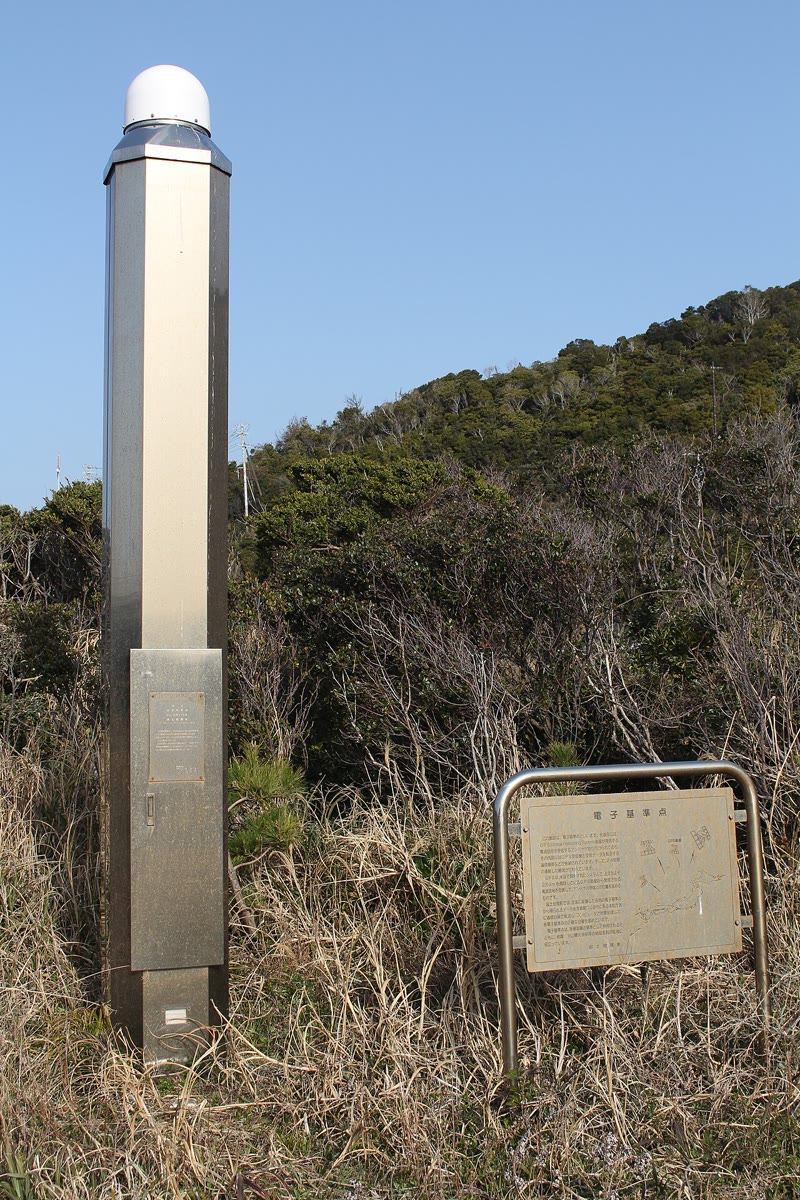
\includegraphics[width=\linewidth]{images/book3/b1-gnss-station.jpg}

{\scriptsize محطة دائمة في اليابان، وهوائيها تحت القبة (Alpsdake, CC BY-SA 4.0).}
\end{minipage}
\end{inthefield}

تعطي سرع المحطات داخل صفيحتين متجهةً لأويلر خاصةً بهما، مستقلةً عن السجل الجيولوجي. فبالنسبة إلى أوراسيا بالنسبة إلى أمريكا الشمالية، تتنبأ هذه المتجهة بمقدار \qty{17.0}{mm.yr^{-1}} في أيسلندا، أي أقل بنحو \qty{8}{\percent} من \qty{18.6}{mm.yr^{-1}} المتوسطة على \qty{3.16}{Myr} (الشكل أعلاه). والوتر بين ريكيافيك وستافانغر، وكلاهما على جزء مستقرّ من صفيحته، يطول بمقدار \qty{17.5}{mm.yr^{-1}}؛ فمتجهة الأقمار الصناعية تتنبأ بمقدار \qty{17.1}{mm.yr^{-1}}، والجيولوجية بمقدار \qty{18.6}{mm.yr^{-1}}. وعبر شمال الأطلسي يتفق معدّل قيس على مدى بضعة عقود مع معدّل متوسط على ثلاثة ملايين سنة في حدود العُشر: فهناك تتحرّك الصفائح اليوم تقريبًا كما تحركت لملايين السنين.
% ledger: morvel:gps-eu-na, morvel:eu-na, ngl:reyk, ngl:stas (chord rates computed in calc/ch12.py)

وداخل منطقة الحدّ تكون الصورة أقل بساطة، لأن المحطات تتحرّك بأكثر من الصفائح. فأكثر من عُشر أيسلندا يقع تحت أغطية جليدية، ومعظمها يفقد كتلته منذ نحو 1890: \omterm{def:b1:layered-earth:layers}{فالقشرة} تحته ترتفع كلما خفّ الحمل، وتتحرّك أفقيًا بعيدًا عن الجليد المتقلّص. والمحطة في هوفن، على الساحل الجنوبي الشرقي قرب أكبر غطاء جليدي، ترتفع بمقدار \qty{12.9}{mm.yr^{-1}}.
% ledger: spaans:iceland-gia, ngl:hofn

\section{التمارين}

خذ $R = \qty{6371}{km}$ في كل مكان.

\begin{exercise}[$\star$]\label{exo:b1:plate-kinematics:1}
\omterm{def:b1:plate-kinematics:euler-pole}{متجهة أويلر} لأوراسيا بالنسبة إلى أمريكا الشمالية معدّلها \qty{0.210}{\degree\per\Myr}. (أ) حوّله إلى \unit{rad.yr^{-1}} وإلى \unit{rad.s^{-1}}. (ب) كم تستغرق دورة كاملة؟ (ج) احسب $\omega R$ بوحدة \unit{mm.yr^{-1}}.
% ledger: morvel:eu-na
\end{exercise}

\begin{exercise}[$\star$]\label{exo:b1:plate-kinematics:2}
بالمتجهة نفسها، احسب السرعة النسبية للصفيحتين عند \ang{30} و\ang{60} و\ang{90} من \omterm{def:b1:plate-kinematics:euler-pole}{قطب أويلر}. أين على طول حدّ الصفيحتين يكون الانتشار أسرع ما يمكن؟
\end{exercise}

\begin{exercise}[$\star$]\label{exo:b1:plate-kinematics:3}
استمرّت الحقبة الفرعية العادية جاراميلو من \qty{1.072}{Ma} إلى \qty{0.988}{Ma}. (أ) ما عرض الخط الذي تصنعه على كل جانب من حيد معدّله النصفي \qty{50}{mm.yr^{-1}}؟ و\qty{10}{mm.yr^{-1}}؟ (ب) ما العرض الكلي للخط الذي تصنعه الحقبة العادية الحالية، التي بدأت منذ \qty{0.781}{Ma}، على حيد معدّله النصفي \qty{10}{mm.yr^{-1}}؟
% ledger: iodp:gpts2004
\end{exercise}

\begin{exercise}[$\star$]\label{exo:b1:plate-kinematics:4}
على قطاع عبر حيد، تقع الحافة الحديثة لشذوذ الحقبة C2An، البالغ عمره \qty{2.581}{Ma}، على بعد \qty{66}{km} غرب المحور و\qty{64}{km} شرقه. احسب المعدّلين النصفيين والمعدّل الكامل. هل الانتشار متماثل؟
% ledger: iodp:gpts2004
\end{exercise}

\begin{exercise}[$\star\star$]\label{exo:b1:plate-kinematics:5}
تقع نقطة على حيد غاكيل، في المحيط المتجمد الشمالي، عند \ang{85}~ش و\ang{0}~ق. احسب بعدها الزاوي عن \omterm{def:b1:plate-kinematics:euler-pole}{قطب أويلر} بين أوراسيا وأمريكا الشمالية (\ang{61.8}~ش، \ang{139.6}~ق، \qty{0.210}{\degree\per\Myr}) ومعدّل الانتشار هناك. قارنه بالمعدّلات المقاسة \qtyrange{11}{12}{mm.yr^{-1}}.
% ledger: morvel:eu-na
\end{exercise}

\begin{exercise}[$\star\star$]\label{exo:b1:plate-kinematics:6}
عند \omterm{def:b1:plate-kinematics:triple-junction}{المفصل الثلاثي} للأزور، عند \ang{39.44}~ش و\ang{29.83}~غ، احسب (أ) البعد الزاوي عن \omterm{def:b1:plate-kinematics:euler-pole}{قطب أويلر} بين أوراسيا وأمريكا الشمالية، (ب) معدّل الانتشار، (ج) \omterm{def:b1:spherical-astronomy:horizontal}{سمت الحركة النسبية}. (د) ما الاتجاه الذي تتنبأ به للصدوع التحويلية في الحيد الذي يقع مباشرة شمال المفصل؟
% ledger: morvel:eu-na, morvel:azores
\end{exercise}

\begin{exercise}[$\star\star$]\label{exo:b1:plate-kinematics:7}
(أ) اكتب متجهتي أويلر $\vec\omega_{\mathrm{EU\,NA}}$ (\ang{61.8}~ش، \ang{139.6}~ق، \qty{0.210}{\degree\per\Myr}) و$\vec\omega_{\mathrm{NB\,NA}}$ (\ang{79.2}~ش، \ang{40.2}~ق، \qty{0.233}{\degree\per\Myr}) بمركباتهما الديكارتية، بوحدة \unit{\degree\per\Myr}. (ب) استنتج $\vec\omega_{\mathrm{NB\,EU}}$ وقطبها ومعدّلها. (ج) لماذا تُعدّ هذه أفضل طريقة لمعرفة حركة النوبة بالنسبة إلى أوراسيا؟
% ledger: morvel:eu-na, morvel:nb-na
\end{exercise}

\begin{exercise}[$\star\star$]\label{exo:b1:plate-kinematics:8}
لنجعل $\vec e_x$ يشير إلى \ang{0}~ش و\ang{0}~ق، و$\vec e_y$ إلى \ang{0}~ش و\ang{90}~ق، و$\vec e_z$ إلى القطب الشمالي. بصيغة رودريغ، احسب صورة $\vec e_x$ (أ) بالدوران بزاوية \ang{90} حول $\vec e_z$ يليه الدوران بزاوية \ang{90} حول $\vec e_x$؛ (ب) بالدورانين نفسيهما بالترتيب المعكوس. (ج) ماذا يعني ذلك لإعادة بناء المواضع الماضية لصفيحة؟
\end{exercise}

\begin{exercise}[$\star\star$]\label{exo:b1:plate-kinematics:9}
تلتقي ثلاث صفائح A و B و C عند مفصل من ثلاثة حيود. وبالنسبة إلى A، تتحرّك الصفيحة B بمعدّل \qty{30}{mm.yr^{-1}} نحو الشرق، والصفيحة C بمعدّل \qty{40}{mm.yr^{-1}} نحو الجنوب. (أ) ارسم مثلث السرع. (ب) احسب سرعة C بالنسبة إلى B وسمتها. (ج) ما اتجاه الحيد بين B و C إذا كان ينتشر عموديًا على محوره؟
\end{exercise}

\begin{exercise}[$\star\star\star$]\label{exo:b1:plate-kinematics:10}
(أ) أثبت أن أثر المصفوفة $R$ لدوران بالزاوية $\alpha$ حول أي محور هو $1 + 2\cos\alpha$. (ب) المصفوفة
\[
  R = \begin{pmatrix} 0 & 0 & 1\\ 1 & 0 & 0\\ 0 & 1 & 0\end{pmatrix}
\]
متعامدة ومحدّدها $1$. أوجد محورها بعرض وطول جغرافيين، وزاويتها. (ج) تحقّق من جوابك بتطبيق $R$ على $\vec e_x$ و$\vec e_y$ و$\vec e_z$.
\end{exercise}

\begin{exercise}[$\star\star\star$]\label{exo:b1:plate-kinematics:11}
قبل تحديد المواقع بالأقمار الصناعية كانت أقطاب أويلر تُستخلص من اتجاهات الصدوع التحويلية. (أ) أثبت أن \omterm{def:b1:plate-kinematics:euler-pole}{قطب أويلر} يقع على \omterm{def:b1:spherical-astronomy:spherical-triangle}{الدائرة العظمى} المارّة بنقطة من صدع تحويلي والعمودية على الصدع هناك، وأن القطب يقع إذن على امتداد $\vec t_1\times\vec t_2$، حيث $\vec t_1$ و$\vec t_2$ متجهتا وحدة على امتداد صدعين تحويليين من الحدّ نفسه.
(ب) تتّجه الصدوع التحويلية بسمت \ang{95} قرب مفصل الأزور الثلاثي (\ang{39.44}~ش، \ang{29.83}~غ)، وبسمت \ang{103} في أيسلندا (\ang{64.5}~ش، \ang{18}~غ). والمتجهة الأفقية للوحدة عند \omterm{def:b1:spherical-astronomy:geographic}{العرض الجغرافي} $\varphi$ والطول $\lambda$، الموجَّهة نحو \omterm{def:b1:spherical-astronomy:horizontal}{السمت} $\beta$، هي $\sin\beta\,\vec e +
\cos\beta\,\vec n$، مع $\vec e = (-\sin\lambda, \cos\lambda, 0)$ و$\vec n =
(-\sin\varphi\cos\lambda, -\sin\varphi\sin\lambda, \cos\varphi)$. حدّد القطب. (ج) ما مدى دقة تحديد القطب بصدعين تحويليين؟
% ledger: morvel:eu-na
\end{exercise}

\begin{exercise}[$\star\star\star$]\label{exo:b1:plate-kinematics:12}
الموضع الشرقي لمحطة، كل ثلاثة أشهر طيلة ثلاث سنوات، هو (بالمليمترات، ابتداءً من $t = 0$):
\begin{center}\small
\begin{tabular}{l*{13}{c}}
\hline
$t$ (yr) & 0 & 0.25 & 0.5 & 0.75 & 1 & 1.25 & 1.5 & 1.75 & 2 & 2.25 & 2.5 & 2.75 & 3\\
$x$ (mm) & 4 & 5 & 6 & 15 & 24 & 25 & 26 & 65 & 74 & 75 & 76 & 85 & 94\\
\hline
\end{tabular}
\end{center}
وهو يتألّف من حركة ثابتة، وتذبذب موسمي، وقفزة ناتجة عن زلزال. (أ) احسب السرعة من الموضعين الأول والأخير. (ب) احسب الفروق التسعة بين موضعين يبعد أحدهما عن الآخر سنةً بالضبط، ووسيطها. (ج) بيّن لماذا يكون وسيط الفروق السنوية تقديرًا متينًا للسرعة الثابتة، ومتى يفشل.
\end{exercise}

\section{مسألة: انشقاق أيسلندا}

\begin{problem}[{مسألة نهاية الأسبوع: انفتاح شمال الأطلسي عبر أيسلندا، مقاسًا بثلاث طرق}]
\label{pb:b1:plate-kinematics:1}
% values: calc/ch12.py (Part II profile invented for the problem; real Euler
% vectors, chron ages and station velocities)
% ledger: morvel:eu-na, morvel:nb-na, iodp:gpts2004, ngl:reyk, ngl:stas, ngl:hofn
تقع أيسلندا على الحيد الأطلسي الأوسط، بين الصفيحة الأمريكية الشمالية غربًا والصفيحة الأوراسية شرقًا. خذ $R = \qty{6371}{km}$، ولحركة أوراسيا بالنسبة إلى أمريكا الشمالية، \omterm{def:b1:plate-kinematics:euler-pole}{متجهة أويلر} بقطبها عند \ang{61.8}~ش و\ang{139.6}~ق ومعدّلها \qty{0.210}{\degree\per\Myr}.

\medskip
\noindent\textbf{الجزء الأول --- متجهة الصفيحة.}
\begin{enumerate}
  \item حوّل المعدّل إلى \unit{rad.yr^{-1}}، واحسب $\omega R$ بوحدة \unit{mm.yr^{-1}}.
  \item احسب المسافة الزاوية $\Delta$ من القطب إلى مركز أيسلندا، \ang{64.5}~ش و\ang{18}~غ.
  \item استنتج \omterm{def:b1:plate-kinematics:spreading-rate}{معدّل الانتشار الكامل} عبر أيسلندا الذي تتنبأ به متجهة الصفيحة.
  \item احسب \omterm{def:b1:spherical-astronomy:horizontal}{سمت القطب} كما يُرى من أيسلندا، وسمت حركة أوراسيا بالنسبة إلى أمريكا الشمالية.
  \item حلّل هذه السرعة إلى مركبتيها الشرقية والشمالية.
  \item على حيد غاكيل، عند \ang{86}~ش و\ang{60}~ق، ما المعدّل الذي تعطيه المتجهة نفسها؟ ولماذا يكون الحدّ هناك أبطأ بكثير؟
\end{enumerate}

\noindent\textbf{الجزء الثاني --- الخطوط المغناطيسية.}
يعطي قطاع مغناطيسي لسفينة عبر حيد ريكيانيس، جنوب غرب أيسلندا قرب \ang{63}~ش و\ang{23}~غ، مُجرى في اتجاه الانتشار، المسافات التالية من المحور إلى ثلاثة حدود حقب (قطاع وُضع لهذه المسألة):
\begin{center}\small
\begin{tabular}{lccc}
\hline
الحدّ & العمر (Ma) & المسافة غرب المحور (km) & المسافة شرق المحور (km)\\
\hline
قاعدة C1n & \mbox{\textdir TLT 0.781} & \mbox{\textdir TLT 9.7} & \mbox{\textdir TLT 10.1}\\
الحافة الحديثة للحقبة C2An & \mbox{\textdir TLT 2.581} & \mbox{\textdir TLT 26.8} & \mbox{\textdir TLT 27.3}\\
الحافة الحديثة للحقبة C5n & \mbox{\textdir TLT 9.779} & \mbox{\textdir TLT 94} & \mbox{\textdir TLT 97}\\
\hline
\end{tabular}
\end{center}
\begin{enumerate}[resume]
  \item من الحافة الحديثة للحقبة C5n، احسب المعدّلين النصفيين.
  \item استنتج \omterm{def:b1:plate-kinematics:spreading-rate}{معدّل الانتشار الكامل} منذ \qty{9.8}{Ma}.
  \item احسب المعدّل الكامل من الحدّين الأحدث أيضًا. هل تتفق الثلاثة؟ صِف كيف تتغيّر مع عمر الحدّ.
  \item هل الانتشار متماثل؟ وهل يغيّر عدم التماثل المعدّل الكامل؟
  \item على حيد ريكيانيس، تُزاح حدود الخطوط بعيدًا عن المحور بمقدار \qty{5.0}{km} في المجموع، على الجانبين معًا. صحّح المعدّلات الكاملة الثلاثة. لماذا كان التصحيح الأهمّ للحدّ الأحدث؟
  \item ما عرض الخط الذي تصنعه الحقبة الفرعية جاراميلو (\qtyrange{1.072}{0.988}{Ma}) على كل جانب، عند المعدّل النصفي المصحّح؟ قارنه بالإزاحة في السؤال 11. ومع ذلك يُعرف شذوذ جاراميلو بوضوح في قطاعات حيد ريكيانيس، وهو غائب عن حيد غاكيل: ماذا يوحي ذلك؟
  \item تتنبأ متجهة الصفيحة بمقدار \qty{19.0}{mm.yr^{-1}} عند القطاع. قارنه بمعدّلاتك المصحّحة.
\end{enumerate}

\noindent\textbf{الجزء الثالث --- الأقمار الصناعية.}
تقع المحطتان الدائمتان REYK (ريكيافيك، \ang{64.139}~ش و\ang{21.955}~غ) وSTAS (ستافانغر، \ang{59.018}~ش و\ang{5.599}~ق) على الصفيحتين الأمريكية الشمالية والأوراسية. وسرعتاهما المقاستان تجعلان الوتر بينهما يطول بمقدار \qty{17.5}{mm.yr^{-1}}.
\begin{enumerate}[resume]
  \item احسب المسافة الزاوية بين المحطتين، وطول الوتر.
  \item كم يستغرق الوتر ليطول بمقدار متر واحد؟
  \item تُعطي متجهة الصفيحة المحطة STAS سرعةً قدرها \qty{18.9}{mm.yr^{-1}} نحو \ang{114.8} بالنسبة إلى أمريكا الشمالية. \omterm{def:b1:spherical-astronomy:spherical-triangle}{والدائرة العظمى} من REYK تصل إلى STAS متجهةً نحو \ang{123.1}. احسب مركبة السرعة على هذا الاتجاه، ثم الزيادة المتنبأ بها في طول الوتر، الذي يصنع الزاوية $\Delta/2$ مع الأفق عند STAS.
  \item قارن الزيادة المقاسة بالمتنبأ بها. ما الذي قد يفسّر الفرق؟
  \item بالنسبة إلى أمريكا الشمالية، تتحرك REYK بمقدار \qty{1.07}{mm.yr^{-1}} نحو الغرب و\qty{0.97}{mm.yr^{-1}} نحو الجنوب، والمحطة HOFN (هوفن، جنوب شرق أيسلندا) بمقدار \qty{21.12}{mm.yr^{-1}} نحو الشرق و\qty{6.97}{mm.yr^{-1}} نحو الجنوب. احسب سرعة HOFN وسمتها بالنسبة إلى REYK.
  \item قارن بالجزء الأول. وترتفع HOFN أيضًا بمقدار \qty{12.9}{mm.yr^{-1}}. لماذا تكون المحطات داخل أيسلندا مقياسًا رديئًا لحركة الصفيحة؟
\end{enumerate}

\noindent\textbf{الجزء الرابع --- عشرة ملايين سنة، والمفصل الجنوبي.}
\begin{enumerate}[resume]
  \item خلال \qty{10}{Myr}، بأي زاوية تدور أوراسيا بالنسبة إلى أمريكا الشمالية حول القطب؟
  \item كم تقطع نقطة من أوراسيا في وسط أيسلندا على طول دائرتها الصغرى في تلك المدة؟ قارنه بالعرض المصحّح \omterm{def:b1:layered-earth:layers}{للقشرة} المتكوّنة منذ الحافة الحديثة للحقبة C5n في الجزء الثاني.
  \item عند مفصل الأزور الثلاثي، تعطي متجهات الصفائح أوراسيا \qty{22.9}{mm.yr^{-1}} نحو \ang{95.1}، والنوبية \qty{19.2}{mm.yr^{-1}} نحو \ang{103.8}، وكلاهما بالنسبة إلى أمريكا الشمالية. احسب سرعة أوراسيا بالنسبة إلى النوبية.
  \item هل هذا المفصل مستقر؟ وأيّ نوع من الحدود تقتضيه السرعة المذكورة في السؤال 22 بين أوراسيا والنوبية؟
  \item اجمع معدّلات الانفتاح من الأجزاء الأول والثاني والثالث. أيّ منها يتفق؟ وأيّ طريقة تقيس حركة الصفائح في أقصر زمن؟
  \item بأقرب مليمتر في السنة، ما \omterm{def:b1:plate-kinematics:spreading-rate}{معدّل الانتشار الكامل} عبر أيسلندا الذي تعطيه متجهة الصفيحة والخطوط المغناطيسية المصحّحة معًا؟
\end{enumerate}
\end{problem}
